\section{Boxing / Killing}
\subsection{Singleton Boxing / Killing}
\subsubsection{Problem}
\begin{itemize}
    \item Some Classes should have only one instance
    \item The instance must be accessible from a well-known access point 
    \item Subclassing from the Singleton should be possible
    \item Extending the Singleton class must not break existing code
    \item How can be guaranteed that only one oject of a class is instantiated and can globally be accessed?
\end{itemize}
\subsubsection{Solution}
Ensure a class only has one instance and provide a global point of access to it 
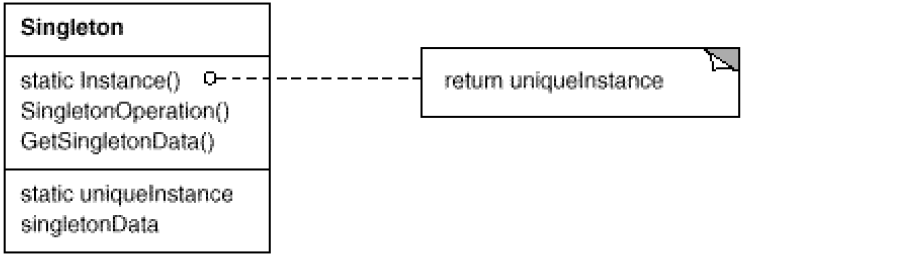
\includegraphics[width=\linewidth]{./img/singleton.png}
\subsubsection{Solutions inside Singleton}
\begin{itemize}
    \item Singleton Pattern
    \item Class Factory Method
    \item Lazy Acquisition
    \item Eager Acquisition
\end{itemize}
\subsubsection{Summary}
\textbf{Benefits}
\begin{itemize}
    \item Controlled access to sole instance
    \item Reduced name space
    \item Permits refinement of operations and representation
    \item Permits variable number of instances
    \item More flexible than class operations
\end{itemize}
\textbf{Liabilities}
\begin{itemize}
    \item Introduces a global variable/state
    \item Prevents polymorphism
    \item Carries state until app closes
    \item Restricts unit testing
\end{itemize}

\subsection{Singleton Variation 'Registry'}
\begin{itemize}
    \item More flexible approach
    \item Uses a registry of singletons
    \item Classes registers their singleton in a well-known registry
\end{itemize}
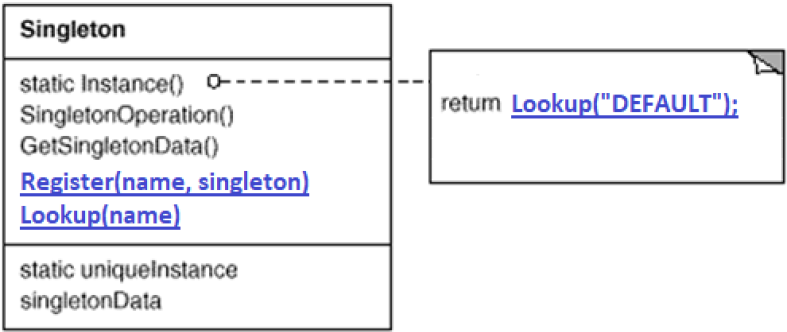
\includegraphics[width=\linewidth]{./img/registry.png}

\subsection{Monostate (Borg) - Killing}
\subsubsection{Problem}
\begin{itemize}
    \item Multiple instances should have the same behaviour
    \item The instances should be simply different names for the same object 
    \item Should have the behaviour of Singleton without imposing the constraint of a single instance
    \item How can two instances behave as though they were a single object?
\end{itemize}
\subsubsection{Solution}
Create a monostate object and implement all member variables as static members 
\begin{lstlisting}
public class Monostate {
    private static int x;
    public int getX() { return x; }
}
\end{lstlisting}
\subsubsection{Summary}
\textbf{Benefits}
\begin{itemize}
    \item Transparency, no need to know about Monostate
    \item Derivability
    \item Polymorphism
    \item Well-defined creation and destruction
\end{itemize}
\textbf{Liabilities}
\begin{itemize}
    \item Breaks inheritance hierarchy
    \item Memory usage
    \item Unable to share Monostate across several tiers
\end{itemize}

\subsection{Service Locator}
\subsubsection{Problem}
\begin{itemize}
    \item Implementation of a global service instance should be exchangeable
    \item It should be possible to execute the service methods on another tier transparently
    \item How could we register and locate global services when one is needed?
\end{itemize}
\subsubsection{Solution}
Implement a service locator that knows how to hold all of the services that an application might need.
\begin{itemize}
    \item Implement the ServiceLocator as a Singleton 'Registry'
    \item ServiceLocator returns \textit{finder} instances, which are used to locate the underlying services
\end{itemize} 
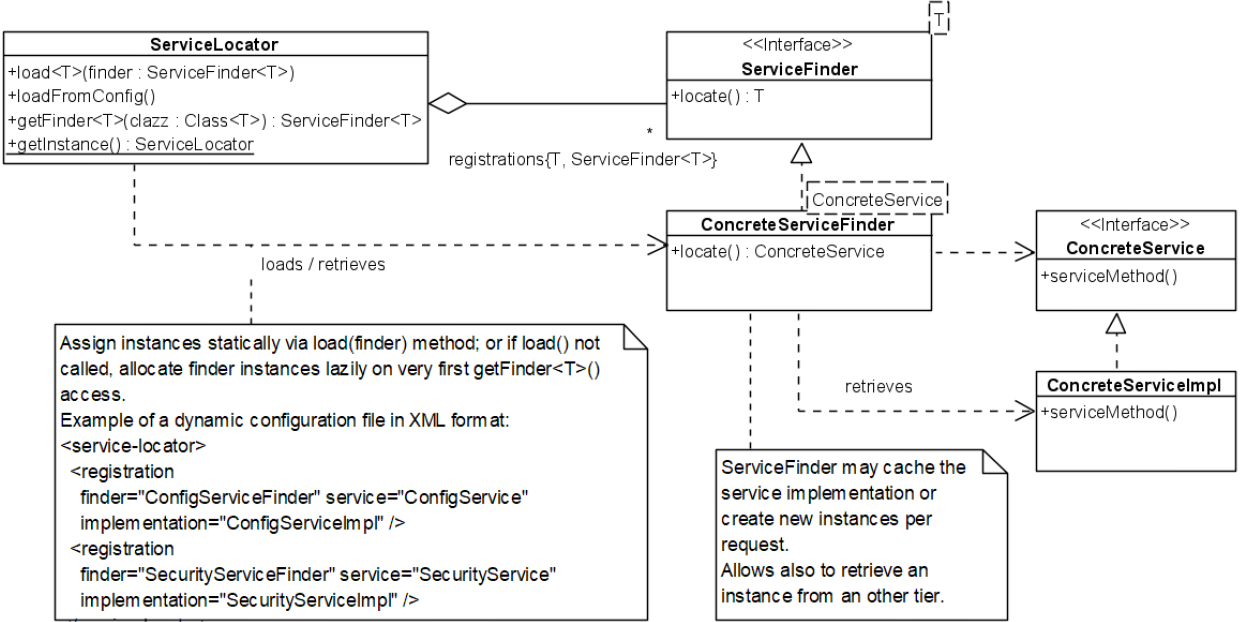
\includegraphics[width=\linewidth]{./img/service_locator.png}
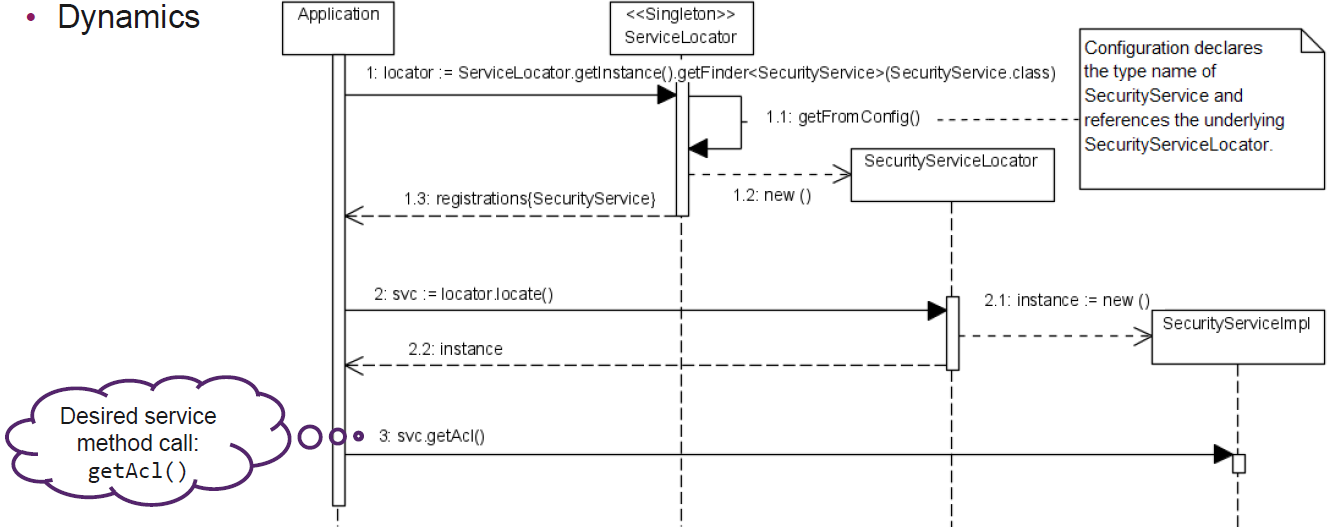
\includegraphics[width=\linewidth]{./img/service_locator_dynamic.png}
\subsubsection{Summary}
\textbf{Benefits}
\begin{itemize}
    \item There is exactly ONE Singleton in the application
    \item ServiceLocator interface strogly rely on abstractness
\end{itemize}
\textbf{Liabilities}
\begin{itemize}
    \item Clients stll rely on a static reference to ServiceLocator class (tight coupling)
    \item No possibility to replace the ServiceLocator 
\end{itemize}

\subsection{Parameterize from Above}
\begin{itemize}
    \item Singleton pattern doesn't provide durability and testability requirements
    \item The application has been layered (horizontally) in a logical manner
    \item How can we povide the required application-wide data to the lower layers without making the data globally accessible?
\end{itemize}
\subsubsection{Solution}
Parameterize each layer from above. Data that affect the behaviour of lower layers should be passed in from the top of the stack.
\begin{itemize}
    \item Pass in configuration parameters and 'known' objects rather than having them global
\end{itemize}
\subsubsection{Summary}
\textbf{Benefits}
\begin{itemize}
    \item No global variables
    \item Implementations of parameterized functionalities are exchangeable
    \item Enforces separation-of-concenrns at architecture level
    \item Reduces coupling between layers
\end{itemize}
\textbf{Liabilities}
\begin{itemize}
    \item Adds more complexity to the system
    \item Contexts must be passed through the whole app stack
    \item Fragile Bootstrapper: app must be wired completely at startup
\end{itemize}

\subsection{Dependency Injection}
\subsubsection{Problem}
\begin{itemize}
    \item User may override implementations of existing app components (e.g. test doubles)
    \item Any Componet within the system can demand an object of a specified interface
    \item The Components should not know anything about the wiring mechanism
\end{itemize}
\subsubsection{Solution}
Introduce a DI Container which loads the interfaces and implementation calsses at startup and dynamically instantiates and wires the objects according to the dependency tree.
\begin{itemize}
    \item Central container
    \item Users reference dependencies by the required interfaces
    \item Users apply code annotations 
    \item Clients should not address the container directly
\end{itemize}
\subsubsection{Implementation}
\begin{itemize}
    \item Combine \textit{Service Locator} and \textit{PfA}
    \item Container class must not be statically referenced by clients
\end{itemize}
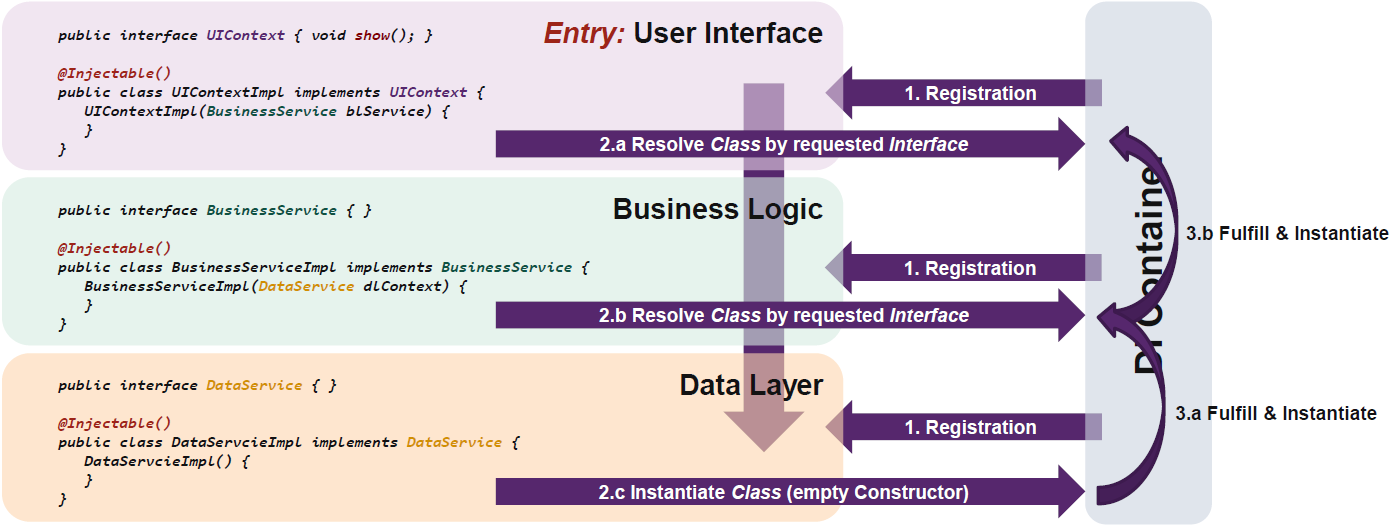
\includegraphics[width=\linewidth]{./img/di_impl.png}
\subsubsection{Summary}
\textbf{Benefits}
\begin{itemize}
    \item Reduces coupling
    \item Contracts between classes are based on interfaces
    \item Suports open/closed principle
    \item Allows flexible replacement of an implementation
\end{itemize}
\textbf{Liabilities}
\begin{itemize}
    \item Adds black magic to the system
    \item Debugging the object dependency tree may become hard
    \item Recursive dependencies are hard to find and may prevent the sytem from startup
    \item Relies on reflection and can result in a performance hit
\end{itemize}
\subsubsection{Discussion}
\textbf{Relation Singleton - DI}
\begin{itemize}
    \item Some injected Dependencies may be singletons
    \item DI Container implementation may be based on 'registry' singleton
\end{itemize}
\textbf{Improvement of DI over Service Locator}
\begin{itemize}
    \item Client classes dont depend directly on the DI Container
    \item Less coupling between DI Container and Component
\end{itemize}

\subsection{Flyweight}
A single pattern for both \textbf{sharing} and \textbf{creation}
\subsubsection{Problem}
\begin{itemize}
    \item Storage costs are high because of the sheer quantity of objects
    \item Many objects bay be replaced by relatively few shared objects
    \item The objects do not depend on object identity
    \item How can multiple copies of a identical constant object be avoided?
\end{itemize}
\subsubsection{Solution}
Use sharing to support large numbers of fine-grained objects efficiently
\begin{itemize}
    \item Flyweight manager maintains instantiated flyweights
    \item Flyweights must be immutable (readonly)
    \item Context information is often maintained by parent object
\end{itemize}
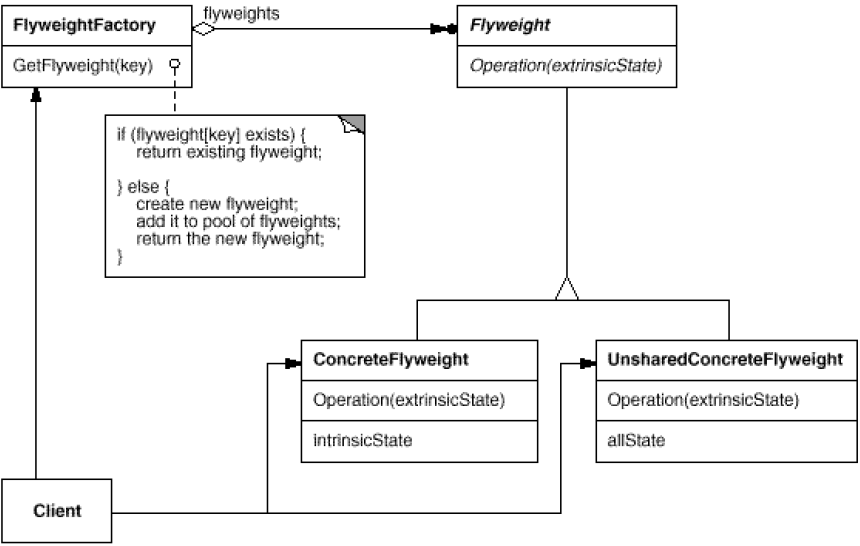
\includegraphics[width=\linewidth]{./img/flyweight.png}
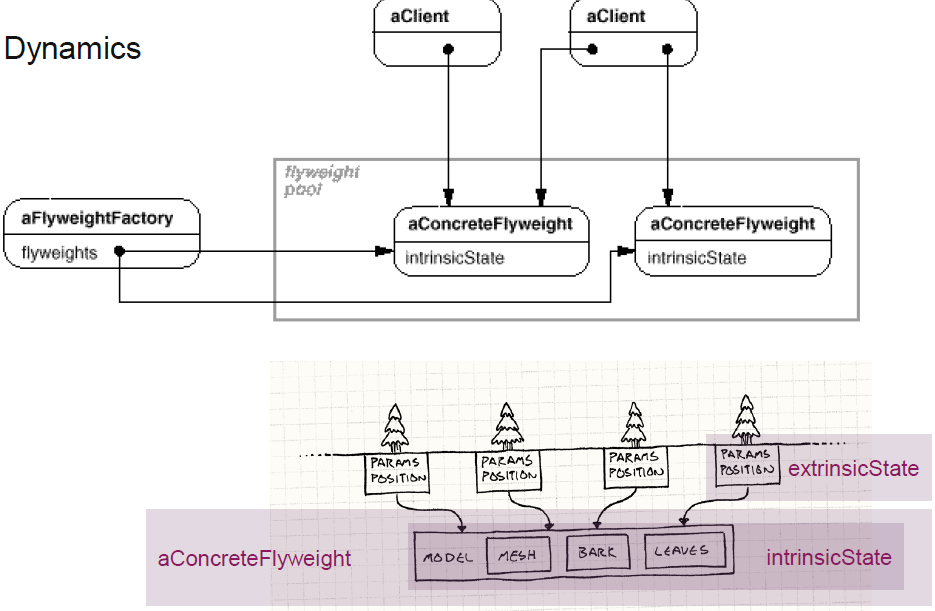
\includegraphics[width=\linewidth]{./img/flyweight_dynamic.png}
\subsubsection{Solutions inside Flyweight}
\begin{itemize}
    \item Composite
    \item Immutable Value
    \item Pooling
    \item Class Factory Method
    \item Lazy Acquisition
    \item Eager Acquisition
\end{itemize}
\subsubsection{Summary}
\textbf{Benefits}
\begin{itemize}
    \item Reduction of the total number of instances (space savings)
\end{itemize}
\textbf{Liabilities}
\begin{itemize}
    \item Can't rely on object identity
    \item May introduce run-time costs
\end{itemize}

\subsection{Pooling (Boxing)}
\subsubsection{Problem}
\begin{itemize}
    \item A fast and predictable access to resources should be provided
    \item Wastage of CPU cycles in repetitious acquisition / release should be avoided
    \item Acquisition / release complexity should be minimized
    \item How can expensive acquisition and release of resources be avoided by recycling resources that are no longer needed?
\end{itemize}
\subsubsection{Solution}
Manage multiple instances of one type of resource in a pool. This pool of resources allows for reuse of released resources.
\begin{itemize}
    \item A resource pool manages resources and gives them to the users
    \item Resource providers, such as OS, owns and manages the resources
\end{itemize}
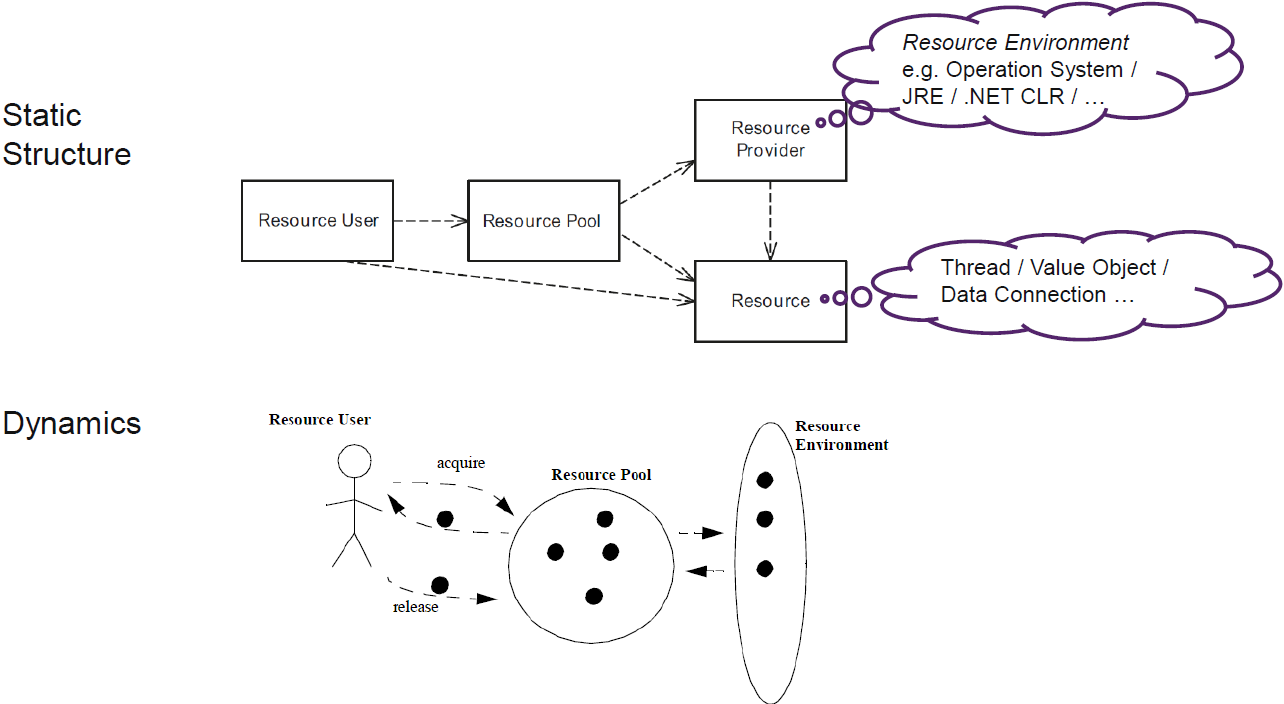
\includegraphics[width=\linewidth]{./img/pooling.png}
\subsubsection{Implementation}
\begin{itemize}
    \item Define the maximum number of resources that are maintained by the pool
    \item Decide between \textit{eager} and \textit{lazy} Acquisition
    \item Determine resources recycling/eviction semantics
\end{itemize}
\subsubsection{Summary}
\textbf{Benefits}
\begin{itemize}
    \item Performance of app
    \item Simplified release and acquisition of resources
    \item New resources can be created dynamically
\end{itemize}
\textbf{Liabilities}
\begin{itemize}
    \item Certain overhead
    \item Acquisition requests must be synchronized to avoid race conditions
\end{itemize}
\subsubsection{Discussion}
\textbf{Pattern that can be combined with Pooling}
\begin{itemize}
    \item Pool acts as mediator
\end{itemize}
\textbf{Relation of Flyweight and Pooling}
\begin{itemize}
    \item Flyweight implements a pool with immutable resources statically
\end{itemize}
\textbf{Is immutability of named resources key?}
\begin{itemize}
    \item No
\end{itemize}
\textbf{Difference between pooling and caching}
\begin{itemize}
    \item Caching is about handling resources with identity, pooling does not
    \item All resources in a pool are equal
    \item Caching only manages object lifetime in cache, not of objects themselve
\end{itemize}